\documentclass{article}
\usepackage{amsmath,amssymb,graphicx,hyperref}
\usepackage{float}

\title{Speeding Up Matrix Multiplication with Machine Learning}
\author{Manan Bhatia}
\date{\today}

\begin{document}

\maketitle

\section{Introduction}
The basic operation of matrix multiplication serves as required in various areas including machine learning and computer science together with computer graphics and scientific simulations. The standard approach to matrix multiplication enables execution at a cubic speed \( O(N^3) \) when the square matrices have dimensions N. The algorithm optimisation requires improvement for large-scale systems because matrix multiplications serve as vital components of neural networks and transformer architectures in deep learning applications.

More efficient algorithms, such as Strassen's algorithm, demonstrates that the potential faster algorithms are possible, including the Copper-Winograd algorithm. However, the research for continuous faster algorithms has only been done by manual process, constrained by human intuition and vast combinatorial nature of practical solutions.

Through research presented in \textit{“Discovering Faster Matrix Multiplication”} it is found out that reinforcement learning technique serves as a method to extend previous work through accelerated mathematical exploration of matrix multiplication. The reinforcement learning agent AlphaZero serves as a basis for AlphaTensor to determine optimal tensor decompositions in finite factor spaces by playing a single-player game. The automated approach detected both standard and new algorithms which proved better than traditional methods for smaller matrix dimensions.

The research expands previous work by studying matrix multiplication mathematics while implementing AlphaZero-inspired reinforcement learning models to evaluate their achieved performance.
\begin{figure}[ht]
    \centering
    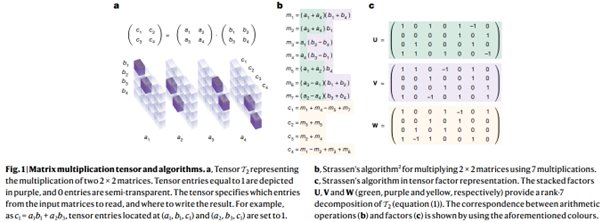
\includegraphics[width=0.6\linewidth]{Picture1.png}
    \caption{Tensor representation of matrix multiplication as a rank-3 tensor. Lower-rank decompositions reduce scalar multiplications. (Source: AlphaTensor paper)}
    \label{fig:tensor-representation}
\end{figure}

\section{Literature Review}
The search for enhanced matrix multiplication algorithms has proven challenging throughout many years in fields of mathematics and computer science. Research studies found ways to decrease the \( N^3 \) scalar multiplication requirement for matrix multiplication by exploiting mathematical structures in the algorithm.

The foundation for improving matrix multiplication processes came from classical methods. The time complexity reached approximately \( O(N^{2.81...}) \) through Strassen's algorithm by converting two \( 2 \times 2 \) matrix multiplication into 7 recursive subproblems rather than 8. 
Coppersmith-Winograd algorithm developed this methodology to achieve matrix multiplication complexity at\(  O(N^{2.376}) \). The state-of-the-art matrix multiplication algorithms currently reach an \( O(N^{2.37}) \) complexity level but actual practical applications tend to use Strassen's method as an economical alternative for medium-scale matrices.

The process of understanding matrix multiplication uses tensor decomposition as an essential mathematical tool. The matrix multiplication operation can be understood as a rank-3 tensor but requires finding the most compact rank representation. The conversion to lower-rank expression requires fewer multiplication operations across scalars. The matrix multiplication tensor of size \( 2 \times 2 \times 2 \) finds its rank-7 decomposition through Strassen's algorithm. Through tensor decomposition researchers gain a unified perspective for both existing algorithm analysis and new algorithm discovery hence becoming an optimal method for optimisation research.

The application of reinforcement learning methods for mathematical discovery opens new possibilities in research. AlphaZero proved that software which links reinforcement learning to self-play with Monte Carlo Tree Search routing could reach superhuman levels in complicated games of Go and Chess. The article modified this framework to develop algorithm discovery along with AlphaTensor which is a reinforcement learning agent that understands tensor factorisation of matrix multiplication. The AlphaTensor system accomplished both the rediscovery of Strassen's algorithm and the identification of newly discovered algorithms that demonstrated better performance than traditional matrix multiplication methods when applied to small matrix sizes. 
The study demonstrated how RL stands as a forceful method for symbolically understanding matters and creating new algorithms.

The proposed synthesis of classical algorithms and tensor decomposition theory and reinforcement learning serves to expand scientific knowledge in matrix multiplication optimisation. The research will adapt AlphaTensor's reinforcement learning approach to evaluate discovered algorithms for their practical value in transformer computations which require heavy use of matrices.

\section{Methodology}

\end{document}